\documentclass[
  captions=tableheading,
  bibliography=totoc, 
  titepage=firstiscover,
]{scrartcl}

\usepackage{blindtext} %neuer input

\usepackage{longtable} % Tabellen über mehrere Seiten

\usepackage[utf8]{inputenc} %neuer input

\usepackage{scrhack}

\usepackage[aux]{rerunfilecheck} %Warnung falls nochmal kompiliert werden muss

\usepackage{fontspec} %Fonteinstellungen

\recalctypearea{}

\usepackage[main=ngerman]{babel} %deutsche Spracheinstellung

\usepackage{ragged2e} %neuer input

\usepackage{amsmath, nccmath}

\usepackage{amssymb} %viele mathe Symbole

\usepackage{mathtools} %Erweiterungen für amsmath


\DeclarePairedDelimiter{\abs}{\lvert}{\rvert}
\DeclarePairedDelimiter{\norm}{\lVert}{\rVert}

\DeclarePairedDelimiter{\bra}{\langle}{\rvert}
\DeclarePairedDelimiter{\ket}{\lvert}{\rangle}

\DeclarePairedDelimiterX{\braket}[2]{\langle}{\rangle}{
#1 \delimsize| #2
}

\NewDocumentCommand \dif {m}
{
\mathinner{\symup{d} #1}
}


\usepackage[
  math-style=ISO,
  bold-style=ISO,
  sans-style=italic,
  nabla=upright,
  partial=upright,
  warnings-off={
    mathtools-colon,
    mathtools-overbracket,
  },
]{unicode-math}

\setmathfont{Latin Modern Math}
\setmathfont{XITS Math}[range={scr, bfscr}]
\setmathfont{XITS Math}[range={cal, bfcal}, StylisticSet=1]


\usepackage[
  locale=DE,
  separate-uncertainty=true,
  per-mode=reciprocal,
  output-decimal-marker={,},
]{siunitx}

\usepackage[autostyle]{csquotes} %richtige Anführungszeichen

\usepackage{xfrac}

\usepackage{float}

\floatplacement{figure}{htbp}

\floatplacement{table}{htbp}

\usepackage[ %floats innerhalb einer section halten
  section,   %floats innerhalb er section halten
  below,     %unterhalb der Section aber auf der selben Seite ist ok
]{placeins}

\usepackage[
  labelfont=bf,
  font=small,
  width=0.9\textwidth,
]{caption}

\usepackage{subcaption} %subfigure, subtable, subref

\usepackage{graphicx}

\usepackage{grffile}

\usepackage{booktabs}

\usepackage{microtype} %Verbesserungen am Schriftbild

\usepackage[
backend=biber,
]{biblatex}

\addbibresource{../lit.bib}

\usepackage[ %Hyperlinks im Dokument
  german,
  unicode,
  pdfusetitle,
  pdfcreator={},
  pdfproducer={},
]{hyperref}

\usepackage{bookmark}

\usepackage[shortcuts]{extdash}

%\usepackage{warpcol}


\begin{document}
    \title{V601 Frank-Hertz-Versuch}
    \author{  
    Tobias Rücker\\
    \texorpdfstring{\href{mailto:tobias.ruecker@tu-dortmund.de}{tobias.ruecker@tu-dortmund.de}
    \and}{,} 
    Paul Störbrock\\
    \texorpdfstring{\href{mailto:paul.stoerbrock@tu-dortmund.de}{paul.stoerbrock@tu-dortmund.de}}{}
    }
    \date{Durchführung: 07.07.2020, Abgabe: 14.07.2020  \vspace{-4ex}}
\maketitle
\thispagestyle{empty}

\newpage
\tableofcontents
\thispagestyle{empty}
\newpage

% Ziel %%%%%%%%%%%%%%%%%%%%%%%%%%%%%%%%%%%%%%%%%%%%%%%%%%%%%%%%%%%%%%%%%%%%%%%%%%%%%%%%%%%%%%%%%%%%%%%%%%%%%%%%%%%%%%%%%%%%%%%%%%%%%%%%%%%%%%%%%%%%%%%%%%%%%%%%%%%%%%%%%%%%%%%%%%%%%%%%%%%%%%%%%%%%%%%%%%%%%%%%%%%%%%%%%

\setcounter{page}{1}
\section{Ziel}\justifying
Die Kenntnis über die innere Struktur der Atome bildet für die verschiedensten Bereiche
der Physik wie die Festkörperphysik eine wichtige Rolle. Da Atome quantisiert sind können
Elektronen nur ganz bestimmte Energiewerte annehmen. Der Übergang vom Grundzustand in den
ersten angeregten Zustand wird nun mithilfe des Frank-Hertz-Versuches bestimmt.

% Theorie %%%%%%%%%%%%%%%%%%%%%%%%%%%%%%%%%%%%%%%%%%%%%%%%%%%%%%%%%%%%%%%%%%%%%%%%%%%%%%%%%%%%%%%%%%%%%%%%%%%%%%%%%%%%%%%%%%%%%%%%%%%%%%%%%%%%%%%%%%%%%%%%%%%%%%%%%%%%%%%%%%%%%%%%%%%%%%%%%%%%%%%%%%%%%%%%%%

\section{Theorie}\justifying
Der Frank-Hertz-Versuch gehört zu den Elektronenstoßexperimenten. Bei diesen 
wechselwirken Elektronen mit Atomen, wobei durch den Energieverlust der Elektronen 
auf den Energieübergang zurückgeschlossen werden kann.\\
\begin{figure}[H]
    \centering
    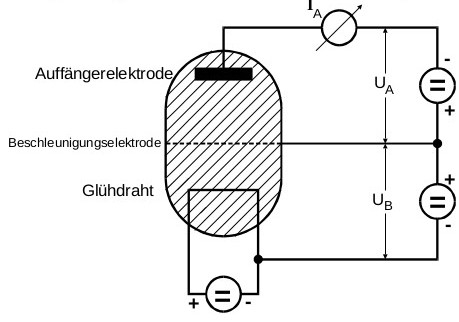
\includegraphics[width=0.8\textwidth]{images/theo_aufbau.jpg}
    \caption{
        Theoretischer Aufbau des Frank-Hertz-Versuchs \cite{V601}.\\
        Bei dem Frank-Hertz-Versuch ist ein evakuiertes Gefäß mit Quecksilbergas gefüllt.
        Ein Glühdraht an einer Spannungsquelle emittiert dabei Elektronen, welche durch die Beschleunigungselektrode
        mit der Beschleunigungsspannung $U_B$
        beschleunigt werden und dann mit den Atomen wechselwirken. Wenn die Elektronen
        dann noch genügend Energie haben um das Gegenfeld der Auffängerelektrode zu überwinden,
        werden sie vom Amperemeter gemessen. 
    } 
    \label{fig:1}
\end{figure}
\leftside{Der} Versuch selbst besteht
dabei aus einem evakuierten Gefäß in dem ein Tropfen Quecksilber spontan verdampft. 
Dieser verdampft so weit bis in dem Gefäß der Gleichgewichtsdruck $p_{sät} $ erreicht ist.
Dieser Druck hängt von der Temperatur im Gefäß ab:
\begin{align}
    p_{sät}(T) = 5,5\cdot 10^7 \exp \left(\frac{-6876}{T} \right) \label{eq:1} \quad \text{(p in mbar, T in K)} \text{\cite{V601}}
\end{align}
Die Elektronen für den Versuch stammen aus einer Glühkathode, wobei die Elektronen
idealerweise monoenergetisch sind. Diese werden durch eine netzförmige Elektrode
mit positiver Gleichspannung $U_B$ beschleunigt. Bei der Wechselwirkung mit 
den Atomen können dann 2 Fälle auftreten. Zum einen können die Elektronen eine
zu geringe Energie besitzen, sodass diese nur elastische Stöße mit den Quecksilberkernen
erzeugen. Der Energieübertrag ist dabei aufgrund des Masseunterschieds vernachlässigbar.
Einzig die Richtungsänderung ist hier entscheidend.\\
Im zweiten Fall haben die Elektronen mindestens die Energie des Übergangs vom Grundzustand
in den ersten angeregten Zustand
\begin{align}
    E=E_1 -E_0 . \label{eq:2} \text{\cite{V601}}
\end{align}
Hierbei ist $E_0$ die Energie des Grundzustands und $E_1$ die Energie des ersten ageregten Zustands.
Nach kurzer Zeit geht das Atom dann wieder unter Aussendung eines Lichtquants in den Grundzustand zurück.
Die Elektronen gelangen danach zu einer Auffängerelektrode, an die eine Gegenspannung $U_A$ 
anglegt wird. Dadurch können nur Elektronen gemessen werden, deren Energie, welche von der 
Geschwindigkeit senkrecht zur Elektrode abhängig ist, größer als das des Gegenfeldes ist.
Wird nun die Beschleunigungsspannung gegen den Auffängerstrom bei kostanter Gegenspannung
aufgetragen, kann dies theoretisch wie folgt aussehen:
\begin{figure}[H]
    \centering
    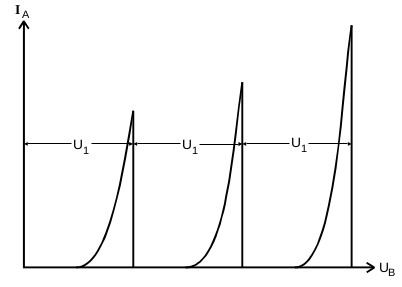
\includegraphics[width=0.7\textwidth]{images/kurve.jpg}
    \caption{
        Theoretischer Verlauf einer idealen der Frank-Hertz-Kurve\cite{V601}.\\
        Bei der Frank-Hertz-Kurve ist die Beschleunigungsspannung gegen den
        Auffängerstrom bei einer festen Gegenspannung aufgetragen. Der Verlauf
        zeigt, dass mit steigender Spannung die Stromstärke erstmal stärker wird,
        bis die Elektronen die Energie des Übergangs vom Grundzustand zum ersten angeregten
        Zustand $U_1$ erreichen. Da fällt die Kurve schlagartig auf 0 ab, da alle Elektronen
        mit den Atomen wechselwirken. Bei weiterer Erhöhung steigt die Kurve weiter an
        bis eine Spannung von 2 $U_1$ erreicht wird. Das wiederholt sich periodisch.
    } 
    \label{fig:2}
\end{figure}
\leftside{Bei} steigender Spannung steigt der Auffängerstrom erstmal an, bis die Elektronen genügend
Energie haben, um das Quecksilber anzuregen. Dann fällt die Stromstärke schlagartig ab.
Dies wiederholt sich dann immer wieder, wobei die Amplituden dabei immer größer werden.
Abstand zweier Maxima ist dabei
\begin{align}
    U_1 = \frac{1}{e_0} (E_1 -E_0) \label{eq:3}. \text{\cite{V601}}
\end{align}
Hier ist $e_0$ die Elementarladung.\\
Die Abbildung \ref{fig:2} liefert hierbei nur eine idealisierte Darstellung des Verlaufs.
Der tatsächliche Verlauf verändert sich durch einige Aspekte des Experiments.
Zum einen bestehen Glühdraht und Beschleunigungskathode aus verschiedenen Materialien,
wodurch das Potential zwischen diesen nicht genau die Beschleuigungsspannung ist.
Bei dem Frank-Hertz-Versuch wird die Austrittsarbeit des Materials $\Phi _g$ der Glühkathode
um einiges kleiner als die der Beschleuigungskathode $\Phi _B$.
Das Verhältnis der Potentiale lässt sich graphisch durch folgende Abbildung darstellen:
\begin{figure}[H]
    \centering
    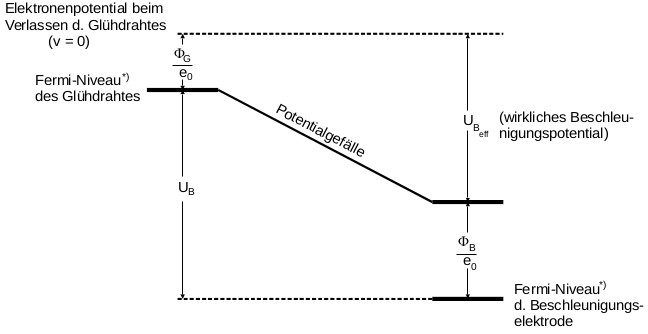
\includegraphics[width=0.8\textwidth]{images/potential.jpg}
    \caption{
        Darstellung des Potentialgefälles zwischen Beschleunigungselektrode und Glühdraht \cite{V601}.\\
        Aufgrund unterschiedlicher Materialien haben Glühdraht und Beschleunigungselektrode
        eine unterschiedliche Austrittsarbeit $\Phi _G$ bzw. $\Phi _B$. Die Austrittsarbeit des
        Glühdrahts ist dabei geringer als die der Beschleunigungselektrode. Dadurch ist die eigentliche
        Beschleunigungsspannung $U_{B,eff}$.
    }
    \label{fig:3}
\end{figure}
\leftside{Damit} ergibt sich für die effektive Beschleuigungsspannung
\begin{subequations}
\begin{align}
    U_{B,eff} &= U_B - \frac{1}{e_0} (E_1 -E_0) \label{eq:4a}\text{\cite{V601}},
    \intertext{
        wobei der Term
    }
    K&:= \frac{1}{e_0} (E_1 -E_0) \label{eq:4b}
\end{align}
\end{subequations}
als Kontaktpotential bezeichnet wird.\\
Zudem besitzen alle Elektronen nicht die gleichen Energien aufgrund der Fermi-Dirac-Verteilung.
Die Verteilung der Energien ist dabei temperaturabhängig und sorgt dafür, dass
die Elektronen unterschiedliche Anfangsgeschwindigkeiten besitzen. Damit gibt es keinen
unstetigen Abfall, wie in Abbildung \ref{fig:2}, sondern es fällt zu einem Minimum ab
und steigt dann wieder an. \\
Zudem sorgt die Ablenkung der Elektronen bei den elastischen Stößen, wenn diese zwischen Beschleunigungsspannung
und Auffängerelektrode stattfinden, dafür, dass deren Geschwindigkeitskomponente senkrecht zur Elektrode
verändert wird. Dadurch wird die Kurve verbreitert und abgeflacht.\\
Damit viele Elektronen mit dem Gas wechselwirken, muss die freie Weglänge
um einen Faktor 1000-4000 mal kleiner als der Abstand von der Kathode zur Beschleunigungselektrode sein.
Die freie Weglänge kann über den bereits erwähnten Sättigungsdampfdruck nach der folgenden Formel reguliert werden
\begin{align}
    \bar w [cm] = \frac{0,0029}{p_{sät}} \;\text{[p in mbar]}. \label{eq:5} \text{\cite{V601}}
\end{align}



% Versuchsaufbau + Versuchsdurchführung %%%%%%%%%%%%%%%%%%%%%%%%%%%%%%%%%%%%%%%%%%%%%%%%%%%%%%%%%%%%%%%%%%%%%%%%%%%%%%%%%%%%%%%%%%%%%%%%%%%%%%%%%%%%%%%%%%%%%%%%%%%%%%%%%%%%%%%%%%%%%%%%%%%%%%%%%%%%%%%%%%%%%%%%%%%%%%%%%%%%%%%%%%%%%%%%%%

\section{Versuchsaufbau und Versuchsdurchführung}\justifying
Der Aufbau für den Frank-Hertz-Versuch wird in der folgenden Abbildung dagestellt:
\begin{figure}[H]
    \centering
    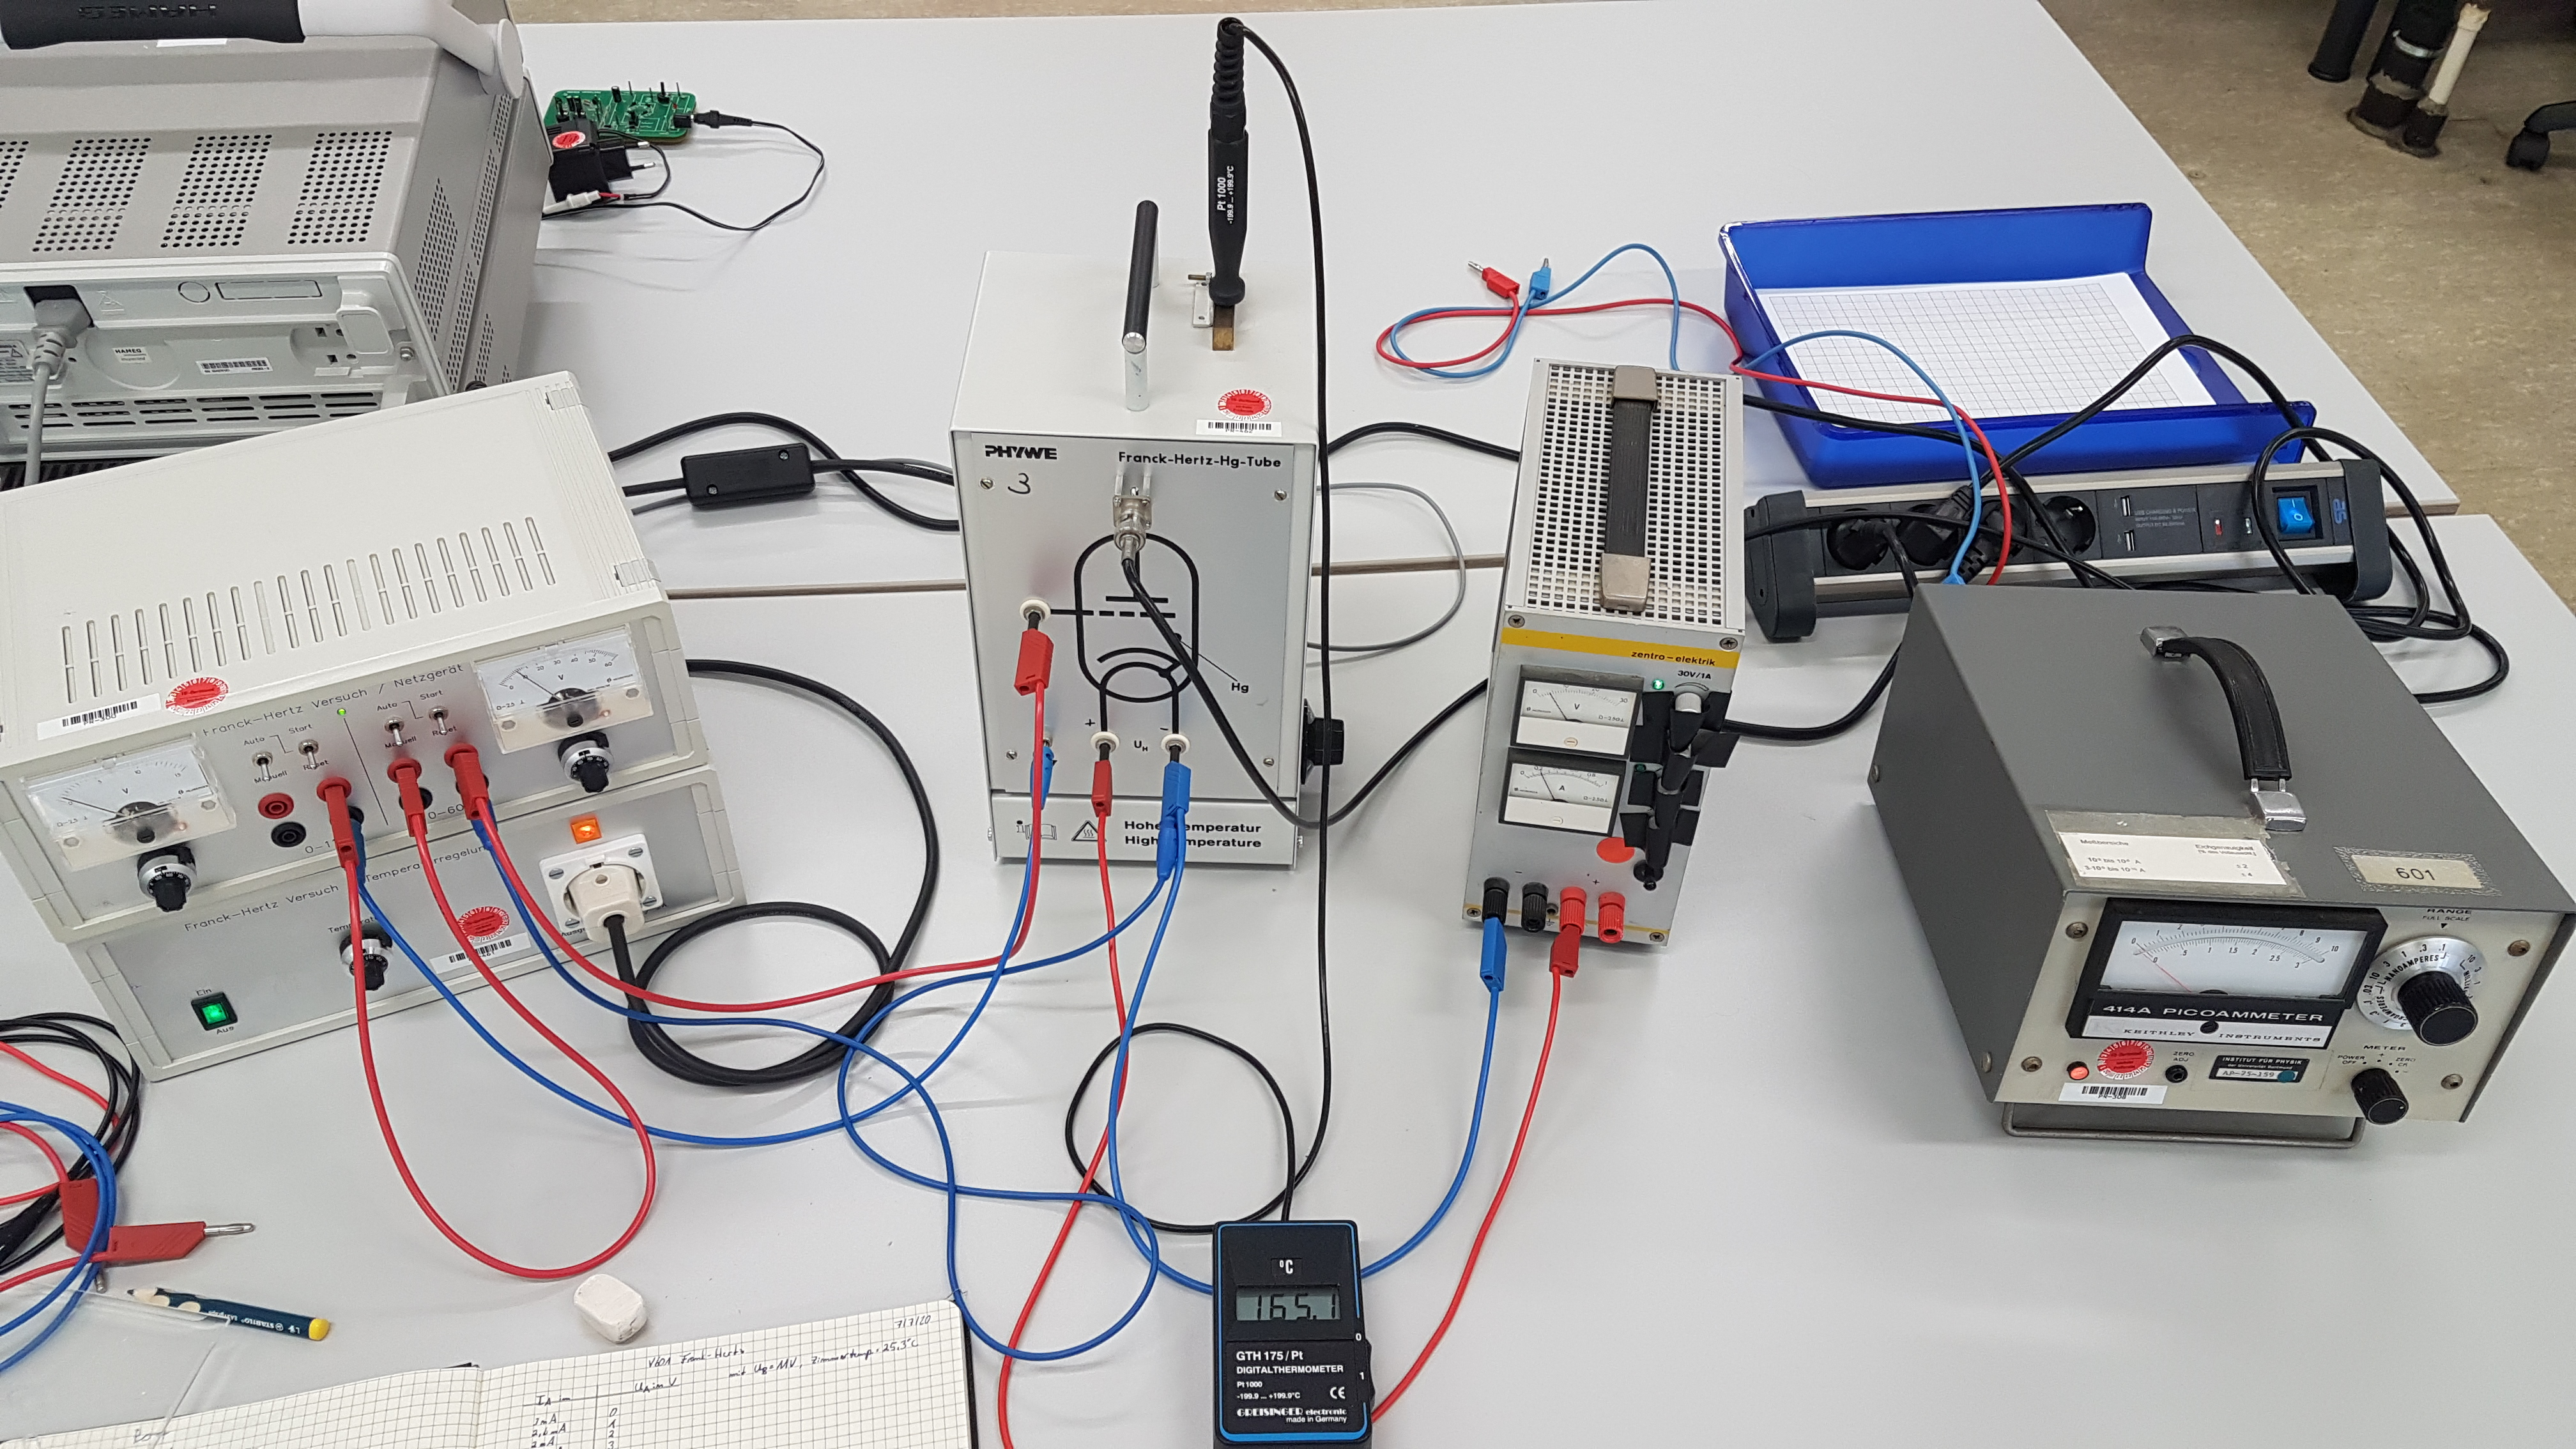
\includegraphics[width=0.8\textwidth]{images/Aufbau.jpg}
    \caption{
        Aufbau des Frank-Hertz-Versuchs.
        Das zweite Gerät von links bildet die evakuierte Glasröhre, in der sich
        das Quecksilbergas mitsamt Glühdraht, Beschleunigungselektrode und Auffängerelektrode
        befindet. Links davon befindet sich das obere Gerät zur Regulierung der beiden Spannungen
        $U_B$ und $U_A$ sowie das untere Gerät zur Erhöhung der Temperatur. Ganz rechts im Bild steht
        das Amperemeter zur Messung des Auffängerstroms $I_A$. Zwischen Amperemeter und
        der Glasröhre befndet sich die Spannungsquelle des Glühdrahts.
    } 
    \label{fig:4}
\end{figure}
\leftside{Das} zweite Gerät von links ist das evakuierte Glasrohr mit Auffängerelektrode, Glühdraht und
Beschleunigungselektrode. Das ganz rechte Gerät ist das Amperemeter, welches den
Auffängerstrom misst. Die ganz linken Geräte sind für die Einstellungen der Spannung und 
die Erhitzung des Glasrohrs zuständig. Das zweite Gerät von rechts ist die Spannungsquelle
des Glühdrahts.\\
Für die Durchführung wird zuerst die Beschleunigungsspannung konstant auf \SI{11}{\volt} eingestellt.
Dann wird bei Zimmertemperatur die Gegenpannung gegen den Auffängerstrom im mesbaren Bereich gemessen.
Daraufhin wird die Temperatur auf den Bereich von 140 - \SI{160}{\celsius} erhöht und die Messung in diesem Bereich wiederholt.\\
Dannach wird die Gegenspannung auf \SI{1}{\volt} gestellt und die Glasröhre auf eine Temperatur von
ungefähr \SI{164}{\celsius} erhitzt. Dann wird die Beschleunigungsspannung gegen
den Auffängerstrom gemessen. Danach wird die Temperatur auf ca. \SI{175}{\celsius} gestellt 
und die Messung wiederholt. Die Temperatur wird dabei möglichst konstant gehalten.


% Auswertung %%%%%%%%%%%%%%%%%%%%%%%%%%%%%%%%%%%%%%%%%%%%%%%%%%%%%%%%%%%%%%%%%%%%%%%%%%%%%%%%%%%%%%%%%%%%%%%%%%%%%%%%%%%%%%%%%%%%%%%%%%%%%%%%%%%%%%%%%%%%%%%%%%%%%%%%%%%%%%%%%%%%%%%%%%%%%%%%%%%%%%%%%%%%%%%%%%

\section{Auswertung}
Alle Plots in der Auswertung werden mit matplotlib \cite{matplotlib} erstellt.
Alle Fehler werden mit uncertainties \cite{uncertainties} und numpy \cite{numpy} berechnet.\\
Der Sättigungsdampfdruck und der Wirkungsquerschnitt für die in der Aufgabe vorkommenden
Temperaturen ist in der folgenden Tabelle dargestellt.
\input{T_table.tex}
\leftside{Der} Sättigungsdampfdruck wird hier mit Gleichung \eqref{eq:1} und der Wirkungsquerschnitt 
mit Gleichung \eqref{eq:5} berechnet.

\subsection{Differentielle Energieverteilung}

Die Tabelle mit den Messwerten für die differentielle Energieverteilung findet sich im Anhang \ref{tab:2}.
Bei den nachfolgenden Plots wird die Gegenspannung $U_A$ gegen die Steigung
aufgetragen. Für die Berechnung der Steigung wird die Differenz der zwei nachfolgenden
y-Werte durch die Differenz der x-Werte gebildet
\begin{align}
    m = \frac{\Delta y}{\Delta x}=\frac{y_2-y_1}{x_2-x_1} \label{eq:6}.
\end{align}

\begin{figure}[H]
    \centering
    \includegraphics[width=\textwidth]{plot_UA.pdf}
    \caption{
        Messung der differentiellen Energieverteilung für eine Temperatur von \SI{298.4}{\kelvin}.
        Aufgetragen ist die Spannung des Gegenfeldes gegen die Steigung, welche aus
        zwei nachfolgenden Werten der Tabelle \ref{tab:2} jeweils gebildet wird.
    } 
    \label{fig:5}
\end{figure}
\begin{figure}[H]
    \centering
    \includegraphics[width=\textwidth]{plot_UA_2.pdf}
    \caption{
        Messung der differentiellen Energieverteilung für eine Temperatur von \SI{418.6}{\kelvin}.
        Aufgetragen ist die Spannung des Gegenfeldes gegen die Steigung, welche aus
        zwei nachfolgenden Werten der Tabelle \ref{tab:2} jeweils gebildet wird.
    } 
    \label{fig:6}
\end{figure}

\subsection{Frank-Hertz-Kurve}

Die Messwerte für die Frank-Hertz-Kurve befindet sich im Anhang in der Tabelle \ref{tab:3}.
Werden die Messwerte graphisch aufgetragen, ergibt sich folgender Plot:

\begin{figure}[H]
    \centering
    \includegraphics[width=\textwidth]{plot_UB.pdf}
    \caption{
        In der Abbildung werden Messwerte der
        Frank-Hertz-Kurve bei den Temperaturen \SI{437.1}{\kelvin} und \SI{448.1}{\kelvin} und einer Gegenspannung von \SI{1}{\volt} dargestellt.
        Die vertikalen Linien in der Graphik zeigen die Orte der lokalen Maxima der Kurve für \SI{448.1}{\kelvin}. Die erkennbaren
        befinden sich bei 30, 36, 41, 46 und \SI{52}{\volt}. Der Abstand zweier 
        Maxima definiert dabei die Übergangsenergie vom Grundzustand zum 1.
        angeregten Zustand.
    }
    \label{fig:7} 
\end{figure}
\leftside{Die} eingezeichneten vertikalen Linien markieren die lokalen Maxima bei den
Messwerten für \SI{448.1}{\kelvin}. Der Abstand zweier Maxima bildet nach 
Abbildung \ref{fig:2} die Spannung U1. Bei Mittelung ergibt sich für E nach Formel \eqref{eq:3}
\begin{align}
    E = \text{\input{U1.tex}}. \label{eq:7} 
\end{align}
Als Wellenlänge ausgedrückt ergibt das
\begin{align}
    \lambda = \frac{h c}{E} = \text{\input{lambda.tex}}  , \label{eq:8} 
\end{align}
wobei h das plank'sche Wirkungsquantum und c die Lichtgeschwindigkeit im Vakuum ist.
Für die Rechnung  werden die Konstanten aus der scipy-Bibiliothek  verwendet.
Der Fehler ergibt sich aus der Gaußschen Fehlerfortpflanzung
\begin{align}
    \Delta \lambda = \sigma _{E}  \frac{h c}{E^2}. \label{eq:9} 
\end{align}



% Diskussion %%%%%%%%%%%%%%%%%%%%%%%%%%%%%%%%%%%%%%%%%%%%%%%%%%%%%%%%%%%%%%%%%%%%%%%%%%%%%%%%%%%%%%%%%%%%%%%%%%%%%%%%%%%%%%%%%%%%%%%%%%%%%%%%%%%%%%%%%%%%%%%%%%%%%%%%%%%%%%%%%%%%%%%%%%%%%%%%%%%%%%%%%%%%%%%%%%

\section{Diskussion}
Bei der Tabelle \ref{tab:1} sind bis auf die Messung bei Zimmertemperatur alle
Messungen mit einem passenden Wirkungsquerschnitt nach der Theorie durchgeführt worden.
Der Abstand a sollte einen Faktor 1000-4000 größer sein, damit möglichst viele Elektronen
bei der passenden Energie wechselwirken. Für die Messung bei Zimmertemeratur werden
weniger Elektronen wechselwirken, da hier der Wirkungsquerschnitt wesentlich geringer ist.\\
Ein Problem in der Auswertung stellt die Bestimmung der differentiellen Energieverteilung dar.
Die aufgenommenen Daten waren sehr klein und nach ein paar Volt nicht mehr mit dem 
Amperemeter zu messen. Dadurch konnte aus diesen Daten kein Kontaktpotential ermittelt werden.
Die Versuchsdurchführung war ursprünglich mit einem XY-Schreiber durchzuführen.
Da dieser aber defekt war mussten Messwerte von Hand aufgenommen werden. \\
Die Übergansenergie aus der Frank-Hertz-Kurve beträgt \SI{5.50+-0.29}{\electronvolt}.
Der relative Fehler für die Übergangsenergie beträgt hierbei
\begin{align}
    U1_{\text{relerr}} = \frac{E-\SI{4.9}{\electronvolt}}{E} =\text{\input{relerr_U1.tex}}. \label{eq:10} 
\end{align}
Der Literaurwert ist dabei aus der Quelle \cite{linsen200926} entommen worden.
Eine Erklärung des relativen Fehlers bietet die stark schwankenden Temperaturen
während der Messung. Es stellte sich als sehr schwierig heraus, diesen konstant zu halten.
Diese Schwankungen haben teilweise 20-\SI{50}{\celsius} betragen. Auch sind Messwerte bei kleineren
Spannungen teilweise nicht messbar gewesen, da sie zu klein waren, um vom Amperemeter 
gemessen werden zu können.


% Literatur %%%%%%%%%%%%%%%%%%%%%%%%%%%%%%%%%%%%%%%%%%%%%%%%%%%%%%%%%%%%%%%%%%%%%%%%%%%%%%%%%%%%%%%%%%%%%%%%%%%%%%%%%%%%%%%%%%%%%%%%%%%%%%%%%%%%%%%%%%%%%%%%%%%%%%%%%%%%%%%%%%%%%%%%%%%%%%%%%%%%%%%%%%%%%%%%%%

\newpage
\printbibliography
\newpage
\section*{Appendix}
\addcontentsline{toc}{section}{Appendix}
\input{UA_table.tex}
\input{UB_table.tex}

\end{document}